\subsection{Propuestas}
Se propone utilizar arquitecturas \aclink{RAG} para mejorar la precisión, ofreciendo al modelo información sobre la generación de consultas \aclink{JQL}. La idea detrás de esto es que, al tener un modelo de recuperación que pueda acceder a una base de conocimiento, el modelo de generación pueda generar respuestas más precisas y acordes al contexto proporcionado. Además, se propone un nuevo conjunto de datos.

Si bien el conjunto de datos inicial era robusto, se ha propuesto un nuevo conjunto, de 100 preguntas, que busca, no solo tener más datos, sino hacerlos más diversos y cambiar en cierto modo las preguntas para cubrir el máximo número de casos posible. Este conjunto de datos se ha pensado durante el desarrollo y las diferentes pruebas lanzadas y también se ha usado como apoyo un dataset existente en \textit{Hugging Face}~\cite{datasetHF}.

A continuación, se describirán las distintas alternativas propuestas para mejorar la precisión del modelo JiraGPT Next.

\subsubsection{Ontología}
Durante el inicio de este trabajo se consultaron artículos como \textit{Sequeda et al.}~\cite{sequeda2023benchmark}, que exploraban la posibilidad de utilizar ontologías en el prompt para mejorar la interpretación de los datos y la generación de consultas SQL, logrando resultados prometedores. Partiendo de esta idea, se propone crear una ontología que represente las reglas que existen en las consultas JQL. La información que se pretende representar en la ontología se ha extraído directamente de la documentación oficial de JIRA, brindada por Atlassian, donde se detallan las reglas que se deben seguir para la creación de consultas JQL~\cite{jiradocs}.

En la figura \ref{fig:diagrama_ontologia} se muestra una visualización de la ontología y las diferentes jerarquías que existen.
\begin{figure}[H]
    \centering
    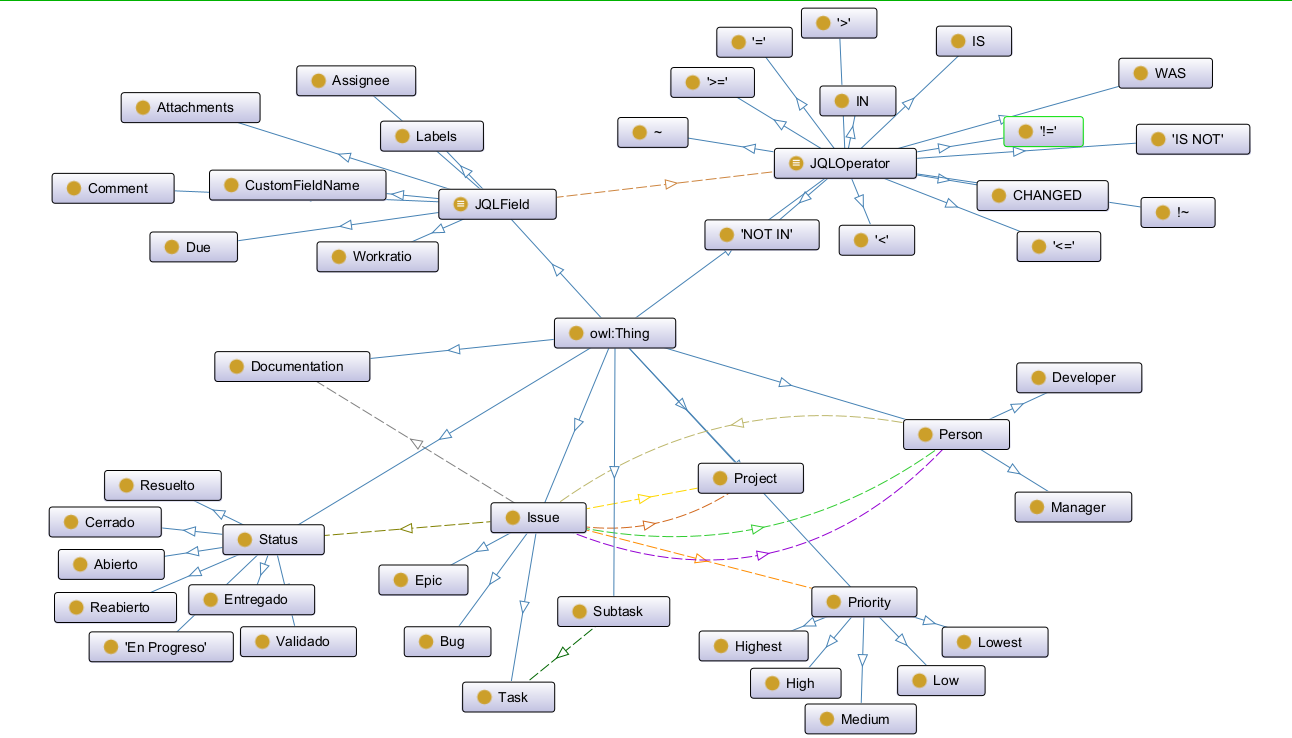
\includegraphics[width=0.95\textwidth]{images/ontologia_visualizacion.png}
    \caption{Ontología representativa de JQL y Jira}\label{fig:diagrama_ontologia}
\end{figure}

Se ha decidido hacer la ontología de esta manera para tratar de representar todas las reglas de JQL aprovechando la semántica de una ontología y la estructura de jerarquía de Jira. Entre las distintas clases, que representan campos, operadores, estados y prioridades, también existen reglas que indican si son compatibles en una consulta, sin embargo, al plasmar la ontología en un diagrama como este no se puede apreciar la semántica de las relaciones. Por ejemplo, la siguiente figura muestra las reglas del campo `Assignee`, indicando qué operadores son soportados por este campo, lo cual en la ontología se describe para todos los campos.

\begin{figure}[H]
    \centering
    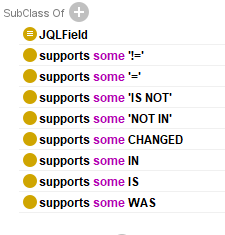
\includegraphics[width=0.335\textwidth]{images/supports_assignee.png}
    \caption{Reglas del campo `Assignee`}\label{fig:assignee_supports}
\end{figure}


La interacción con la ontología representa un reto, ya que una vez definida la ontología, interactuar con ella de manera que el modelo comprenda lo que se representa es complejo. Se ha optado por utilizar el mismo modelo de lenguaje para buscar los posibles campos relevantes dada una pregunta. Por ejemplo, para la pregunta '¿Qué incidencias tiene asignadas Alberto Aróstegui?', se envía al modelo para que responda indicando qué campos son relevantes para esa pregunta, utilizando una plantilla, adjunta en el anexo I, en la que se le exponen todos los campos que hemos descrito en la ontología, el modelo debería responder con el campo Assignee, que es el campo descrito en la ontología que mejor responde a esa pregunta en su respectiva consulta JQL. Una vez se tienen estos campos, se puede consultar la ontología para obtener toda la información que se represente y que sea relevante para la pregunta, como las subclases que tiene, las restricciones que existen con otros campos u operadores o comentarios que se expongan en la ontología sobre ese campo. El siguiente diagrama muestra cómo es el flujo del sistema.

\begin{figure}[H]
    \centering
    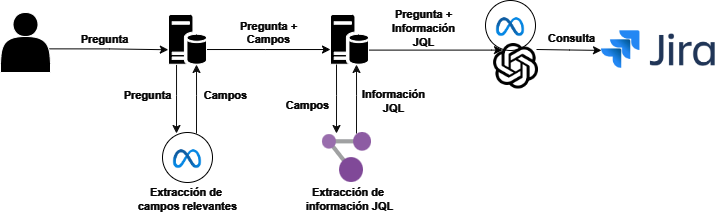
\includegraphics[width=0.95\textwidth]{images/rag_ontologia.png}
    \caption{Diagrama de RAG con ontología}\label{fig:ontologia}
\end{figure}


\subsubsection{Embeddings}
De igual manera que en el diseño de la ontología, se propone capturar la documentación oficial de JIRA en esta base de datos vectorial. Esta base de conocimiento almacena los embeddings de los diferentes descripciones dentro de la documentación. La información que se ha considerado relevante ha sido cada campo/operador/función y sus respectivos ejemplos. De esta manera, dada una pregunta se podrían obtener los embeddings de las palabras y compararlas con los embeddings de la base de datos, de manera que el modelo obtenga ejemplos de campos relevantes para la pregunta del usuario. Las figuras \ref{fig:field} y \ref{fig:examples}, extraídas directamente la documentación oficial de Jira, describen un campo JQL y ofrecen ejemplos de uso.
\begin{figure}[H]
    \centering
    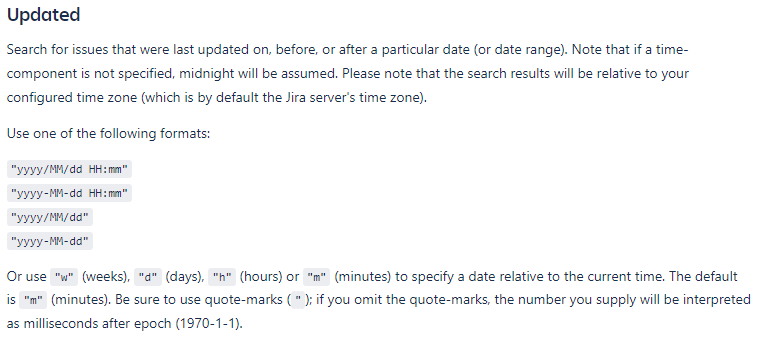
\includegraphics[width=0.95\textwidth]{images/JQL_docs_updated1.png}
    \caption{Campo JQL}\label{fig:field}
\end{figure}
\begin{figure}[H]
    \centering
    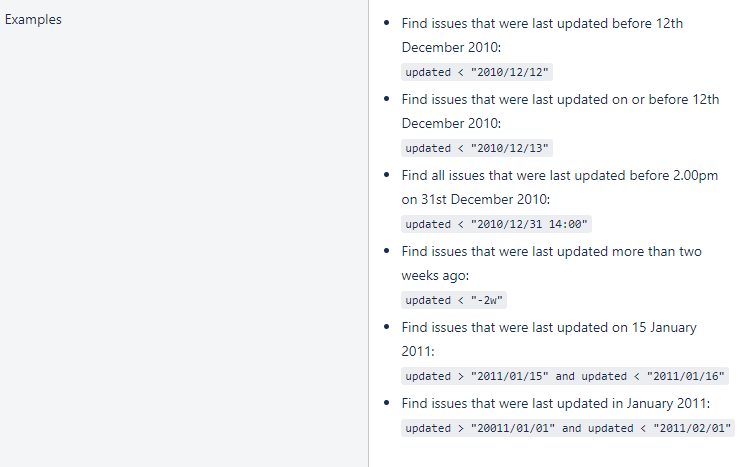
\includegraphics[width=0.95\textwidth]{images/JQL_docs_updated2.png}
    \caption{Ejemplos de uso}\label{fig:examples}
\end{figure}

Para capturar toda la información de la documentación se ha diseñado un programa en Python que realiza técnicas de \textit{web scraping} y recorre las entradas de la documentación extrayendo de las tablas los ejemplos. Una vez hecho esto, se guarda en un archivo de texto que será dividido en diferentes partes para ser procesado por el modelo de embeddings, generando vectores de 1536 dimensiones que representan la información de la documentación de manera numérica. Estos valores de cada dimensión indican una característica de los datos, en caso del texto podría representar conceptos como intenciones o similitudes. De esta manera, oraciones que tengan similitudes, como por ejemplo `incidencias cuyo estado cambió durante agosto` y, de la documentación, el operador `changed` que tiene como ejemplo `Find issues whose status had changed from 'In Progress' back to 'Open'` generarían vectores similares.

Teniendo la pregunta del usuario, se ha de traducir al inglés, ya que la documentación oficial está en inglés y dada una pregunta en castellano la recuperación de información de los embeddings no sería efectiva. Para traducir la pregunta, se utiliza GPT-4o y, dada la pregunta traducida, se hace una búsqueda en la base de datos vectorial, obteniendo los ejemplos más relevantes para la pregunta dada. Esta información se inyecta en el prompt para que el modelo pueda generar una respuesta más precisa. El diagrama en la siguiente figura \ref{fig:embeddings} cómo será la interacción entre el modelo y la base de datos vectorial.

\begin{figure}[H]
    \centering
    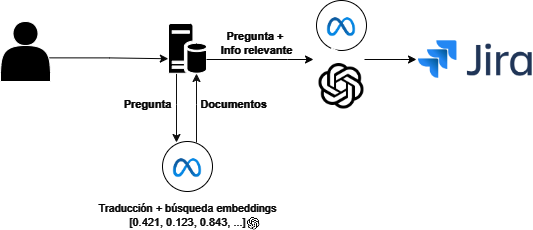
\includegraphics[width=0.95\textwidth]{images/rag_embeddings.png}
    \caption{Diagrama de RAG con embeddings}\label{fig:embeddings}
\end{figure}

\subsubsection{Knowledge Graphs}
Como última propuesta para el trabajo, se ha planteado el uso de Knowledge Graphs para tratar de guiar al modelo en la estructura de la información contenida en la plataforma JIRA de LKS Next-GobTech. La idea detrás de esta propuesta es que, dada la información de Jira en forma de grafo, el modelo podría ser capaz de inferir cómo es la estructura de información de la plataforma Jira de LKS Next-GobTech y generar respuestas que sean más acordes a lo que se busca. Para esto, se ha de crear un Knowledge Graph que contenga la información de Jira de cada proyecto que tenga activo LKS Next-GobTech, por lo que se ha de crear un programa que sea capaz de transformar esa información en un grafo y se pueda ejecutar de manera periódica, con el fin de que el grafo esté actualizado con la información real que se almacena en Jira. Cada proyecto tendrá su grafo y el programa que crea el grafo a partir de la información de la API debería ser ejecutado periódicamente para mantener la información actualizada.

En la figura \ref{fig:desglose_kg} se puede apreciar el desglose de una incidencia representada en el grafo para el proyecto `MFM`, con Arkaitz Carbajo como autor (Reporter) y una persona cualquiera asignada a esta tarea. Además, se puede ver que es una tarea de tipo Tarea (No un bug o un error) y es de tipo `Issue` al ser una incidencia, como todas las demás. Se puede ver que su estado actual es `Abierto`, además, el nodo `MFM-35` contiene como informacion literal las fechas de creación y vencimiento de esta tarea.

\begin{figure}[H]
    \centering
    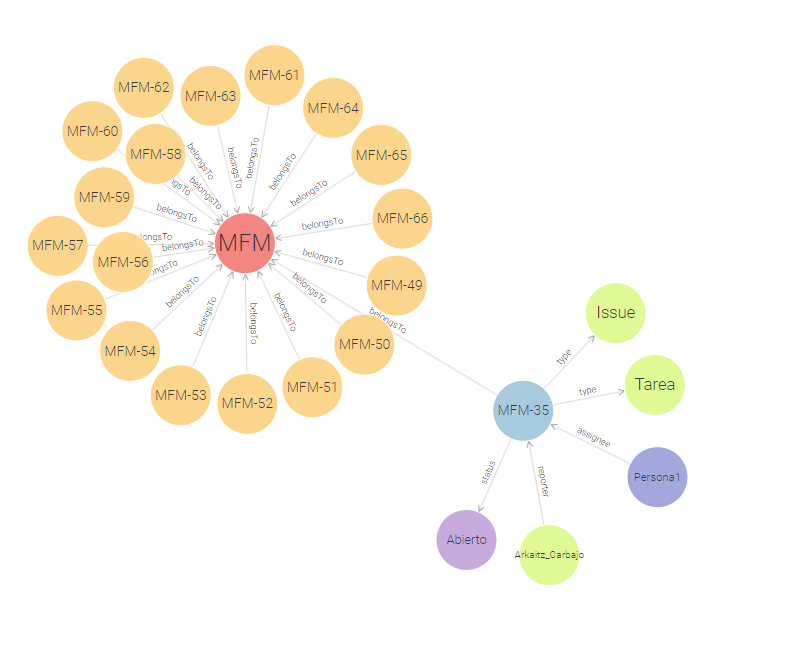
\includegraphics[width=0.95\textwidth]{images/desglose_kg.png}
    \caption{Knowledge Graph para el proyecto MFM, diagrama en GraphDB}\label{fig:desglose_kg}
\end{figure}

El flujo sería el representado en la figura \ref{fig:kg}, donde se muestra cómo, dada una pregunta de un usuario, se extrae información del knowledge graph que se inyectaría en el prompt para que el modelo pueda generar una respuesta con más contexto.

\begin{figure}[H]
    \centering
    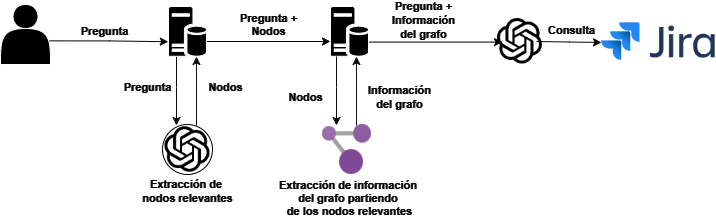
\includegraphics[width=0.95\textwidth]{images/rag_grafo.png}
    \caption{Diagrama de RAG con knowledge graphs}\label{fig:kg}
\end{figure}
